\hypertarget{robotics-frameworks-and-languages}{%
\section{Robotics Frameworks and
Languages}\label{robotics-frameworks-and-languages}}

A \emph{Robotics Framework} is currently a ``catch-all'' term. To most
roboticists it means a collection of tools to support robotics software
development. Typically a framework will provide some form of
interprocess communication and a collection of hardware drivers.
Interprocess communication is either shared memory and semaphore
wrappers or TCP/IP socket support. {[}If these terms don't sound
familiar, we will discuss them later in the text.{]} There are many
simulation systems available. These range from fairly simplistic 2D
single robot with a few obstacles to very sophisticated 3D full physics
engine support systems. It is similar to what is seen in computer
gaming. We will discuss a few of the more popular approaches below.

\hypertarget{player}{%
\subsection{Player}\label{player}}


\includegraphics[width=0.15\textwidth,height=\textheight]{ToolsFigures/player_button_v3.png}

The beginnings of ROS date back to the Player project, which was founded
in 2000 by Brian Gerkey. This model included a hardware-abstracted
robotic system known as the player, which interfaced with its simulated
environment, known as the stage.

\texttt{Player} is a robotics framework. It provides communications and
robot control interfacing. This is open source freely available
software. Player is one of the leaders in the distributed approach to
robotic control software. It provides a network interface to a variety
of hardware devices and systems. Using a client-server approach, it
gives the ability to control any device from any location. This allows
multiple languages and multiple platforms to be used as a single robot
control system; as long as they support sockets (TCP). It is especially
useful in research when the low level software is in C, the sensor
package is in Java and the behavior system is written in Python,
allowing the best tool for the job to be used. Player is still
maintained, but development ceased in 2010 (mostly due to ROS).

\texttt{Stage} is the simulation system that is loosely coupled with
Player. They are separate but have been extensively used together. Stage
is consider a 2.5D (more than 2D but less than 3D) simulation
environment. Stage is oriented towards a world which is described by a
two dimensional map of objects with some height. Fine details in the
\(z\) direction are not modeled so the tool is not designed for
simulation of grasping or manipulation. Stage is a very popular tool for
modeling ground robots (and multiple ground robots). It has options to
be compiled with control code or communicate with Player via the network
interface. In this case, your control code would talk to Player which
interfaces with Stage. The concept is that you develop your control
software interacting with Stage. Then when ready to deploy, you
disconnect Player-Stage and connect Player to the real hardware.

Player-Stage is a great idea. Getting it to compile and run is rather
difficult. Since development has slowed and many developers have moved
on, finding the right combination of Player version, Stage version, OS
version and library collection can be frustrating. When it compiles and
runs, it is a great tool. It can be found at
\url{http://playerstage.sourceforge.net}.

\hypertarget{switchyard}{%
\subsection{Switchyard}\label{switchyard}}

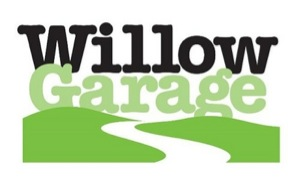
\includegraphics[width=0.15\textwidth,height=\textheight]{ToolsFigures/willow_garage.jpg}

The common API used by player was a major part of the next step on the
road to ROS, the Stanford project known as \emph{Switchyard.}
\texttt{Switchyard} was developed by Morgan Quigley in 2007 under the
Stanford Artificial Intelligence Robot (STAIR) project. Development of
the system was shifted to a Stanford robotics start-up known as
\texttt{Willow\ Garage} in 2008. The platform matured for about 2 years,
and in 2010, Willow Garage released the first version of ROS.

\hypertarget{ros}{%
\subsection{ROS}\label{ros}}

\texttt{ROS}, the \texttt{Robot\ Operating\ System}, is an open source
robotics framework. This project grew out of Player and many of the
lessons learned with Player are found in ROS. ROS provides the
communication system, a filesystem, distribution system and several
thousand packages for device support, robot control, machine vision,
sensor fusion, mapping, localization, etc. ROS was supported by Willow
Garage (robotics company out of Stanford), but now maintained by the
Open Source Robotics Foundation.

As of 2021, ROS (and ROS2) is the dominant open source robotics software
framework. It has seen commerical adoption and has large community
support. The name is a bit misleading in that it is not an operatung
system but more middleware. ROS originally was developed to run on
Ubuntu. With the release of ROS2, MacOS and Windows have basic support.
A real strength is the number of user contributed packages available to
support various sensors and devices, navigation, controls and
localization algorithms, and system support.

As a simulation systme, ROS is still able to connect to Stage however
the current focus is on Gazebo. Gazebo is an open source 3D simulation
envirnoment for robotics (which began life with Player). It includes a
full physics engine such as ODE, Bullet, Simbody, and DART. ROS and
Gazebo are extensions in some sense to Player-Stage. The idea of
developing code in simulation then redirecting to real hardware is
essentially the same.

\hypertarget{osrf}{%
\subsection{OSRF}\label{osrf}}


\includegraphics[width=0.15\textwidth,height=\textheight]{ToolsFigures/osrf_masthead.png}

In 2012, development of ROS began to shift from Willow Garage to the
newly formed, Open Source Robotics Foundation, \texttt{OSRF} also
oversees development of the Gazebo robot simulator, as well as the
annual ROSCon, where ROS developers meet and discuss various ROS-related
topics. Development using ROS still continues at Willow Garage, but the
framework as a whole is developed at OSRF.

\hypertarget{ms-robotics-developer-studio}{%
\subsection{MS Robotics Developer
Studio}\label{ms-robotics-developer-studio}}

Microsoft Robotics Developers Studio, \texttt{MSRDS}, is a full featured
robotics development environment. First released in 2006 and the current
stable release in 2012, made this framework an early player in the
robotics community. It provides support tools for developing
applications, supporting communications, visual authoring and
simulation. MSRDS is a commercial application. The tool includes an
asynchronous runtime environment which supports threading and
interprocess communication. VPL is the Visual Programming Language which
is in the spirit of Visual Studio and Visual Basic. This tool provides a
drag and drop GUI for application development as well as export to C\#.
DSSME is a configuration editor to support application configuration and
distribution. VSE, Visual Simulation Environment provides 3D simulation
with physics. Robotics control software may be developed, simulated and
tested without hardware. No updates have been released since 2012. On
Sept. 22, 2014 Microsoft suspended their robotics division and so no
further development is expected. MSRDS can found at
\url{http://www.microsoft.com/robotics/}.

\hypertarget{webots}{%
\subsection{Webots}\label{webots}}

Like MSRDS, \texttt{Webots} is a full featured robotics development and
simulation environment as well. It is a commercial application and is
more oriented to instruction/simulation than the others described here.
This tool provides a large choice of simulated sensors and hardware.
Robotic control code can be prototyped in simulation and then ported to
hardware for tuning. The goal is to provide a realistic simulation to
reduce development time using their Model, Program, Simulate, Transfer
approach. Unlike MSRDS, Player and ROS; Webots is more of a real physics
engine, with collision detection and dynamics simulation and less of a
robot OS/communications framework. It can be found at
\url{http://www.cyberbotics.com}.

\hypertarget{robotics-programming-languages}{%
\subsection{Robotics Programming
Languages}\label{robotics-programming-languages}}

There is not a ``best'' robotics programming language just as there is
not a best programming language in general. Arguments about a best
language are left to novices attempting to justify the language they
most recently learned. Programming languages are tools like pliers,
screwdrivers and hammers. It depends on what you want to do, what
resources you have available and your personal skill set. Currently C,
C++ and Python are some of the most popular languages in robotics.

The C family is used heavily since it has a small footprint and is very
efficient. C is the major language for embedded systems (C fits on
microcontrollers). Nearly all systems have a C compiler and maybe only a
C compiler.

C++ provides the object oriented approach to a code base and is widely
adopted in industry. Both remain in the most popular programming
language lists even though they have been around for some time.

Python is an object oriented scripting language and is has wide adoption
due to ease of learning, ease of use, and very compact reabable syntax.
Python now is one of the leading languages in high school and college
courses.

Recent languages like Java and C\# are popular when the robot has a full
computer available as a controller. One can even find older languages
like BASIC and FORTH as well. Choice of a language for development will
depend on the available languages, the requirements of the system,
available libraries and support tools, the skills of the developer and
team, and many other details. Having multiple languages deployed may
also be needed since no one language or library can cover the
requirements.

This text will focus on the concepts (mathematics) and algorithms and is
not concenred with integration into a specific environment. This text
will use the Python language which can illustrate the ideas, reasonably
easy to work with, and supports the various numerical operations.
